\documentclass[../../main]{subfiles}

\renewcommand\thesection{\arabic{section}}


\begin{document}

\section{Asking the Right Questions} \label{sec:}

In order to make sense of the data, we need to ask the \emph{right questions}
about the data. Traditionally this is know as an \emph{Algorithm}.

% Figure
% \ref{fig:solvingAProblem} depicts this work flow.
%
% %% TODO: Draw a better figure.
%
% \begin{figure} [H]
%     \centering
%     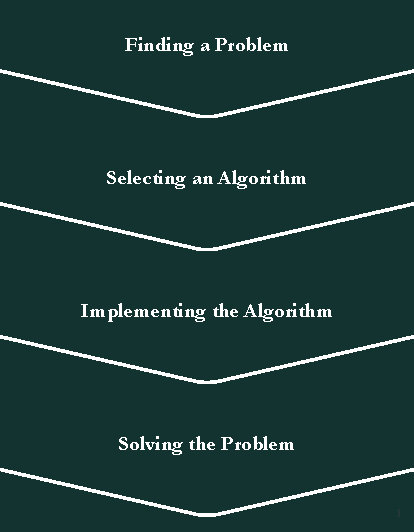
\includegraphics [
%         max width = \IGXMaxWidth,
%         max height = 0.3\textheight,
%         \IGXDefaultOptionalArgs,
%     ] {pics/solving_a_problem.pdf}
%     \captionof{figure} {Traditional way of solving a problem.}
%     \label{fig:solvingAProblem}
% \end{figure}

Once we have a problem, we will analyse the problem then pick an appropriate
\emph{algorithm} that fits the problem. Then we can simply implement the
algorithm and be able to arrive at the solution.

But there is an upper limit this method can take us. What if the problem
that we are trying to solve is really complicated and we can't come up
with a proper algorithm to solve it? In those cases we need to find another
way to solve the problem at hand. But before that let's see some of the
different ways we can model our questions.

\end{document}
